\chapter{ВСТУП}

%Hidden cite for correct bibliography ordering
\nocite{bahvalov-et-al,benerdge-et-al} 

\textbf{Актуальність теми.}

Традиційне хірургічне втручання або відкрита хірургія характеризується відносно великим розтином м'яких тканин. Для 
доступу до органу над яким хірург має провести маніпуляцію також треба зупинити кровотечу спричинену розтином. Ці дії 
проводяться в умовах стерильності, які серйозно обмежують кількість рухів, які виконує лікар. Це зменшує комфорт 
проведення операційного втручання.

З іншої сторони великий розтин дозволяє отримати широкий кут огляду місця провення хірургічної операції. Проте така 
зручність супроводжується суттєвими недоліками:
\begin{itemize}
  \item Збільшення ймовірності інфекції.
  \item Суттєві больові відчуття у пацієнта\textbackslashпацієнтки після операції.
  \item Довший період реабілітації від хірургічного втручанння.
  \item Великий шрам у місці розтину.
\end{itemize}

Головним фактором вищезгаданих недоліків є великий розтин у м'яких тканинах. Тому були створені нові методи 
малоінвазивної хірургії. Суттєва різниця полягає у розмірі отвору через який вводяться хірургічні інструменти. 
Зокрема у лапароскопічній операції, яка є одним із підвидів малоінвазивної хірургії, через отвори утворений в результаті 
проколу м'яких тканин вводяться інструменти. Серед них є ендоскоп, який виводить зображення на монітор і освітлює місце 
проведення операції.

\begin{figure}[h!]
  \centering
  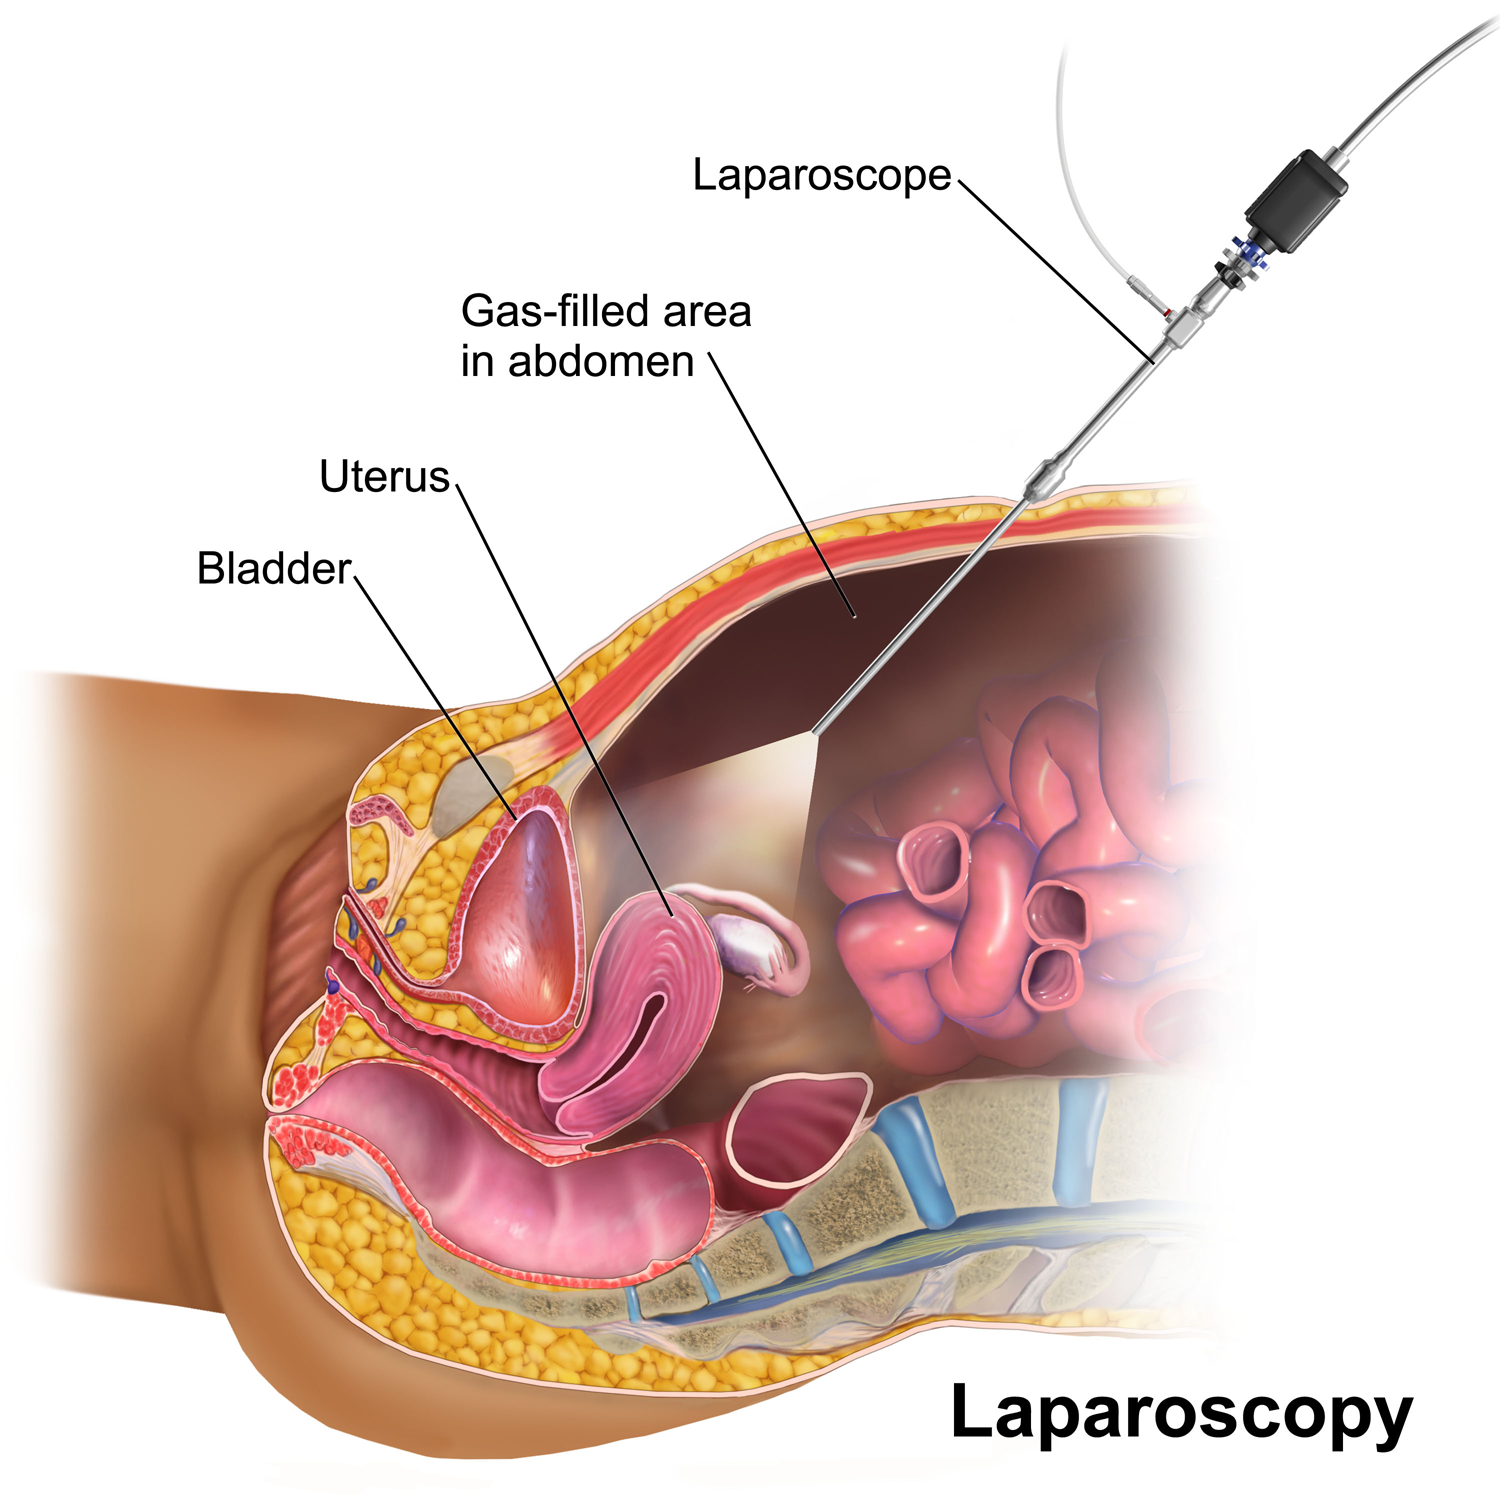
\includegraphics[width=0.4\linewidth]{images/intro_laparoscopy.png}
  \caption{Лапароскопія.}
  \label{fig:intro_laparoscopy}
\end{figure}

Лапароскопічні операції (рис. \ref{fig:intro_laparoscopy}) є кроком вперед проте мають ряд недоліків
\begin{itemize}
  \item Збільшення ймовірності інфекції.
  \item Суттєві больові відчуття у пацієнта\textbackslashпацієнтки після операції.
  \item Довший період реабілітації від хірургічного втручанння.
  \item Великий шрам у місці розтину.
\end{itemize}

Малоінвазивна робото хірургія. 


Більшість елементів сучасного приводу, конструкцій чи побутові речі виготовлені із гетерогенного матеріалу, зокрема із композиційного матеріалу або композиту. Тому виникає потреба у розробці методів, які б дозволяли розраховувати напружено-деформований стан, а також температуру.

Широко вживаними протягом кількох десятиріч методом розв'язування задач такого класу є проекційно-сітковий метод або метод скінчених елементів (МСЕ). Завдяки таким властивостям як розрідженість і симетричність матриць для класу задач у локально-неоднорідних тілах, різні варіанти МСЕ набули популярності.

Із МСЕ цілком успішно може конкурувати, а іноді бути ефективнішим,
велике сімейство методів граничних елементів
(МГЕ) \cite{benerdge-et-al} {[}4{]}{[}6{]}{[}7{]}{[}9{]}{[}12{]}{[}16{]}, які базуються
на ідеях розроблених С.Г.Міхліном{[}19{]}, Н.І.Мусхелішвілі{[}20{]},
В.Д.Купрадзе{[}17{]} та інші. Ці обставині особливо сприяють такі
переваги, як зменшення на одиницю геометричної розмірності задачі,
простота розв'язування для безмежних областей, можливість обчислювати у
лінійних задачах значення шуканих величин у довільній точці без нової
апроксимації, простота дискретизації.

У свою чергу серед класу МГЕ можна виділити такі методи як комплексний
метод граничних елементів (КМГЕ) і метод при граничних елементів (МПГЕ).
На відміну від КМГЕ, який є видозміненим варіантом класичного МГЕ, МПГЕ
базується на більш радикальніших ідеях. У порівнянні із МГЕ, МПГЕ
простіший для реалізації, проте у більшості випадків дає точніші
результати при тих самих затратах обчислювальних ресурсів.

Наукове завдання дисертаційної роботи -- розробка ефективного методу для
розв'язування задач термопружності у композитах є актуальною проблемою.

\textbf{Зв'язок роботи з науковими програмами, планами та
темами.} Робота виконувалась на кафедрі програмування львівського
національного університету імені Івана Франка, а також у інституті
прикладних проблем механіки і математики імені Ярослава Підстригача НАН
України, відділ термомеханіки в рамках держбюджетної теми ``Розробка
аналітико-чисельних методів дослідження напруженого стану неоднорідних
тіл з тепловими та залишковими деформаціями і дефектами структури''.
(!!! Номер теми !!!)

\textbf{Мета роботи та задачі дослідження.} Метою роботи є:

\begin{itemize}
\item
  побудова нових методів розв'язування задач термопружності у композитах
\item
  дослідження ефективності нових методів
\item
  порівняння швидкості збіжності і використання ресурсів із відомими
  методами
\end{itemize}

\emph{Об'єктом} дослідження є композити.

\emph{Предметом} дослідження є нові методи розв'язування задач
термопружності для композитів.

\emph{Методи дослідження.} Для розв'язування поставлених задач
використовується метод поєднання граничних і скінчених елементів.

\textbf{Наукова новизна одержаних результатів.} Наступні
результати отримані у роботі є новими:

\begin{enumerate}
\def\labelenumi{\arabic{enumi}.}
\item
  побудований метод на основі КМГЕ і МСЕ для розв'язування задачі
  теплопровідності у тілах із локальними неоднорідностями
\item
  для тіл із локальними неоднорідностями побудований метод на основі
  МПГЕ і МСЕ для розв'язування задач:

  \begin{enumerate}
  \def\labelenumii{\alph{enumii}.}
  \item
    пружності
  \item
    термопружності
  \end{enumerate}
\end{enumerate}

\textbf{Практичне значення отриманих результаті.} Отримані
результати дозволяють ефективніше розв'язувати актуальні проблеми, які
ставить перед нами народне господарство.

\textbf{Апробація результатів дисертації.} Основні результати
виконаних досліджень доповідалися та обговорювалися на:

\begin{enumerate}
\def\labelenumi{\arabic{enumi}.}
\item
  Восьмій Всеукраїнській науковій конференції (25-27 вересня 2001 р., м.
  Львів) ``Сучасні проблеми прикладної математики та інформатики'';
\item
  Дев'ятій Всеукраїнській науковій конференції (24-26 вересня 2002 р.,
  м. Львів) ``Сучасні проблеми прикладної математики та інформатики'';
\item
  Десятій Всеукраїнській науковій конференції (23-25 вересня 2003 р., м.
  Львів) ``Сучасні проблеми прикладної математики та інформатики'';
\item
  Одинадцятій Всеукраїнській науковій конференції (!!! 2004р., м. Львів)
  ``Сучасні проблеми прикладної математики та інформатики'';
\item
  Дванадцятій Всеукраїнській науковій конференції (4-6 жовтня 2005р., м.
  Львів) ``Сучасні проблеми прикладної математики та інформатики'';
\item
  Науковому семінарі ІППММ НАНУ імені Я.С.Підстригача, присвяченої
  пам'яті Є.Г.Грицька (22 квітня 2003 р., м. Львів);
\item
  Шостій Міжнародній науковій конференції (26-29 травня 2003 р., м.
  Львів) ``Математичні проблеми механіки неоднорідних структур'';
\item
  Семінар інституту прикладних проблем механіки та математики ім. Я.
  Підстригача
\end{enumerate}

У повному обсязі робота доповідалася на семінарі кафедри програмування
львівського національного університету імені Івана Франка.

\textbf{Публікації.} Результати досліджень висвітлені в 4 статтях
у журналах з переліку фахових видань ВАК України, в тому числі у
доповідях НАН України.

\textbf{Особистий внесок здобувача.} Всі результати дисертаційної
роботи отримано здобувачем самостійно.

\textbf{Структура та обсяг роботи.} Дисертація складається із
вступу і шести розділів основної частини, висновків, списку використаної
літератури із 37 найменувань.

У першому розділі описано підходи до розв'язування задач термопружності
і підхід, який був вибраний у даній роботи. Проаналізовано переваги і
недоліки кожного із запропонованих методів.

Другий розділ містить опис двох підходів для розв'язування задачі
теплопровідності. Перший підхід базується на ідеї предиктор-коректор, а
другий -- на рівняннях нев'язки у точках областей локальної
неоднорідності коефіцієнта теплопровідності.

Метод адитивного розчеплення оператора застосований для задачі пружності
для локально-неоднорідного тіла запропонований у третьому розділі. Даний
підхід був апробований для двох методів МГЕ і МПГЕ. Наведено порівняння
чисельних результатів для цих двох методів, а також порівняння методів
по інших критеріях, таких як простота реалізації, точність, діагональне
переважання матриць.

Четвертий розділ містить порівняльний аналіз МГЕ і МПГЕ при розв'язуванні задачі пружності у кусково-однорідному тілі. Наводяться рекомендації щодо застосування даних підходів для розв'язування задач такого класу.

У п'ятому розділі наведено підхід на основі МГЕ і МПГЕ для розв'язування
задачі термопружності у тілі із локально-неоднорідними властивостями
фізичних параметрів.

Програмне середовище Aspirant's Calculations Envinronment (ACE) було
створене для простого і зручного програмування запропонованих методів.
Структура даного середовища описана у шостому розділі. Також дано
рекомендації відносно використання даного середовища для програмування
подібних методів, яке вимагає невеликих зусиль спрямованих тільки на
побудову алгоритму, але не на організацію взаємодії між об'єктами.

\textbf{Усталені домовленості.} У цій праці кома перед індексом
означає похідну по змінній, яка відповідає цьому індексу, тобто
 ${f_{,j} = \partial}{f/\partial}x_{j}$, ${{f_{,ij} = \partial^{2}}{f/\partial}x_{i}\partial x_{j}}{}$,
при цьому викори­стовується німе сумування за індек­сами, які
повторюються.
